\chapter{Конструкторская часть}

В данном разделе будут приведены схемы алгоритма поиск узла в двоичном дереве поиска и требования к программному обеспечению.

\section{Разработка алгоритмов}

На рис. \ref{fig:algo} приведены схемы алгоритма поиск узла в двоичном дереве поиска.


\begin{figure}[h]
	\centering
	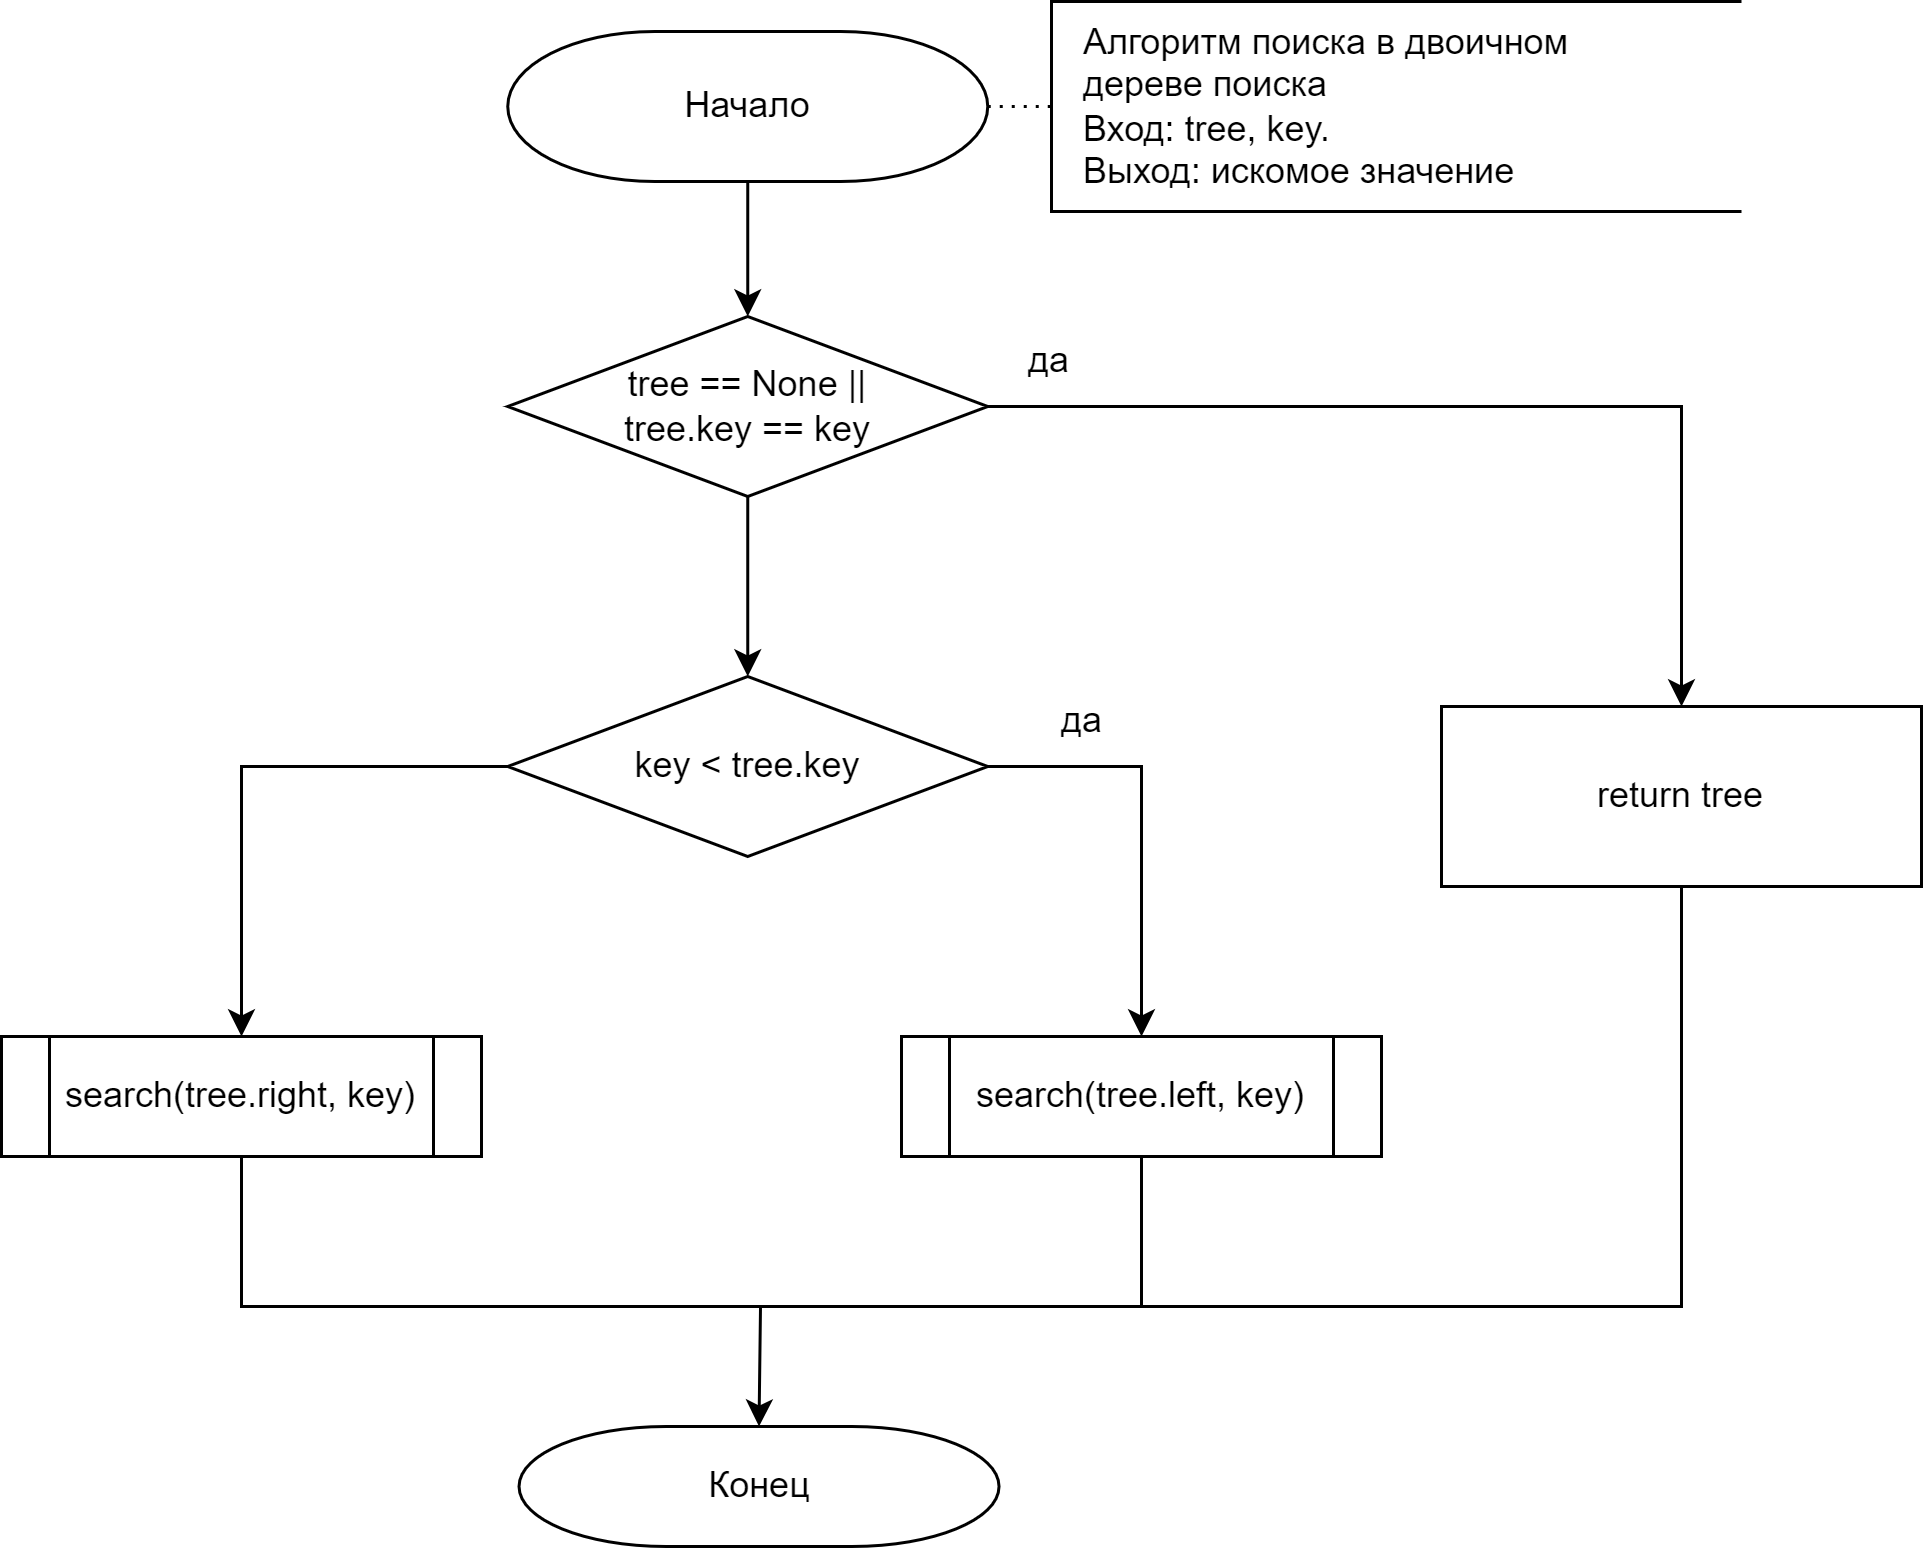
\includegraphics[scale=0.2]{img/algo.png}
	\caption{Схема алгоритма поиск узла в двоичном дереве поиска}
	\label{fig:algo}
\end{figure}

\clearpage

\section{Требования к программному обеспечению}

К программе предъявляются следующие требования:
\begin{itemize}[label=---]
	\item Программа должна предоставлять 2 режима работы: режим поиска целого числа в двоичном дереве поиска несбалансированном и сбалансированном;
	\item В начале работы программы пользователю нужно ввести целое число --- это выбор пункта меню.
\end{itemize}

\section*{Вывод}

В данном разделе приведены схемы алгоритма поиск узла в двоичном дереве поиска и требования к программному обеспечению.

\clearpage